%======================================================================
%----------------------------------------------------------------------
%               XX                              X
%                                               X
%               XX    XXX   XXX   XXX      XXX  X  XXXX
%                X   X   X X   X X   X    X   X X X
%                X   XXXXX XXXXX XXXXX    X     X  XXX
%                X   X     X     X     XX X   X X     X
%               XXX   XXX   XXX   XXX  XX  XXX  X XXXX
%----------------------------------------------------------------------
%  	         A SKELETON FILE FOR IEEE PAPER GENERATION
%----------------------------------------------------------------------
%======================================================================

% first, uncomment the desired options:
\documentclass[%
        %draft,
        %submission,
        %compressed,
        final,
        %
        %technote,
        %internal,
        %submitted,
        %inpress,
        %reprint,
        %
        %titlepage,
        notitlepage,
        %anonymous,
        narroweqnarray,
        inline,
        %twoside,
        ]{ieee}
%
% some standard modes are:
%
% \documentclass[draft,narroweqnarray,inline]{ieee}
% \documentclass[submission,anonymous,narroweqnarray,inline]{ieee}
% \documentclass[final,narroweqnarray,inline]{ieee}

% Use the `endfloat' package to move figures and tables to the end
% of the paper. Useful for `submission' mode.
%\usepackage {endfloat}

% Use the `times' package to use Helvetica and Times-Roman fonts
% instead of the standard Computer Modern fonts. Useful for the 
% IEEE Computer Society transactions.
% (Note: If you have the commercial package `mathtime,' it is much
% better, but the `times' package works too).
%\usepackage {times}

% In order to use the figure-defining commands in ieeefig.sty...
\usepackage{ieeefig}
\usepackage{hyperref}

\begin{document}

%----------------------------------------------------------------------
% Title Information, Abstract and Keywords
%----------------------------------------------------------------------
\title[Continuous Multimodal User Authentication, using soft and hard biometrics]{%
       Continuous Multimodal User Authentication}

% format author this way for journal articles.
% \author[TRIBHUVANESH, SOUMYA AND K.G.SRINIVASA]{%
%       Tribhuvanesh Orekondy
%       \authorinfo{%
%       Department of Computer Science and Engineering,
%       M.S.Ramaiah Institute of Technology, Bangalore, India
%       Phone: \mbox{}, email: \mbox{tribhuvanesh@gmail.com}}
%     \and
%       Soumya Gosukonda\member{Student}
%       \authorinfo{%
%       Department of Computer Science and Engineering,
%       M.S.Ramaiah Institute of Technology, Bangalore, India
%       Phone: \mbox{}, email: \mbox{soumya.gk@gmail.com}}
%     \and
%       and Dr.K.G.Srinivasa\member{}
%       \authorinfo{%
%       Department of Computer Science and Engineering,
%       M.S.Ramaiah Institute of Technology, Bangalore, India
%       Phone: \mbox{}, email: \mbox{tribhuvanesh@gmail.com}}
%   }

% format author this way for conference proceedings
\author[]{%
      Tribhuvanesh Orekondy,
      \authorinfo{%
      Department of Computer Science and Engineering,\\
      M.S.Ramaiah Institute of Technology, Bangalore, India.\\
      email: tribhuvanesh@gmail.com}
    \and
      Soumya Gosukonda,
      \authorinfo{%
      email: soumya.gk@gmail.com}
    \and
      and Dr. K.G.Srinivasa\member{Member}
      \authorinfo{...}
  }

% specifiy the journal name
% \journal{IEEE Transactions on Something, 1997}

% Or, when the paper is a preprint, try this...
%\journal{IEEE Transactions on Something, 1997, TN\#9999.}

% Or, specify the conference place and date.
% \confplacedate{Ottawa, Canada, May 19--21, 1997}

% make the title
\maketitle               

% do the abstract
\begin{abstract}
Static Authentication methods, although providing a rigid and secure framework to this one-time authentication session, do not provide authentication of the user throughout the session. This leaves the possibility of an imposter gaining access in multiple scenarios.\\
The goal of \emph{Continuous Authentication} is to authenticate the user right from the initial stages of log-in through log-out.
This can be implemented by extrapolating the tried-and-tested static authentication techniques thoughout the session.
But, this introduces new challenges, since these "one-time authentication" techniques are computationally expensive, restricts the user's movement and postures in front of the system, require extra expensive hardware and deviates the user from his work-flow.
In these situations, the user no longer remains uninterrupted by the authentication process in the background.\\
This project proposes Continuous Authentication, using login through conventional passwords followed by authentication using two modes - hard and soft biometrics till logout. The hard biometric trait - facial features, is chosen so that the user need not invest in any additional expensive hardware. The noise inherent in the process of face recognition, is managed by using a machine learning algorithm which captures the temporal data and expresses it as confidence. The soft traits are used in phases when this confidence is high to relieve the CPU of comparatively high computation.
\end{abstract}

% do the keywords
\begin{keywords}
Continuous Authentication, Computer Vision, Face recognition, Machine Learning, Support Vector Machine, Biometrics
\end{keywords}

% start the main text ...
%----------------------------------------------------------------------
% SECTION I: Introduction
%----------------------------------------------------------------------
\section{Introduction}
\PARstart Authentication of the user is an important aspect of security that has been implemented over time, in many ways based on the following aspects of a user \cite{Klos00}:

\begin{itemize}
	\item Something the user \emph{knows}: This refers to conventional password based login. Passwords are encrypted and stored in the database.
	\item Something the user \emph{has}: This can refer to tokens that a user possesses which authenticate a user, like an ID card. 
	\item Something the user \emph{is}: This refers to biological or behavioural traits of a user such as fingerprint, facial features or Keystroke Dynamics\cite{mon00}. These traits are enrolled during account creation or during log-in (depending on what type of characteristic feature is being recorded) and are used when the system needs to re-inforce its belief of the user's identity.
\end{itemize}
All of the above have been used in various combinations, for static as well as continuous authentication of a user. \emph{Static Authentication} is the method of authenticating a user, at the time of log-in. Password-based authentication are a popular implementation of this concept. However, passwords can be subjected to being stolen or cracked using various techniques. Also, static authentication methods, in general, do not ensure that the user remains authenticated throughout the session. Therefore, there is need for a system that continually verifies the user's identity, while allowing the user to continue his/her work uninterrupted. Such a system is called a \emph{Continuous Authentication system}.
A lot of research and experimentation has been done in the field of Continuous Authentication \cite{Niin10,Klos00,mon00,turk03,sim07,azz08,azz082}, though it has not been adopted for widespread usage as readily as the Static Authentication systems have been. Continuous Authentication tends to utilize a user's biometric traits for identification, since they can be monitored without distracting the user from his/her work \cite{Klos00}. \emph{Biometric traits} refer to the physiological or behavioural traits of a user that can identify a user, for a session. These traits can be divided into the following two categories:
\begin{itemize}
	\item Hard Biometric traits: These are physical traits of a user that are assumed to be present universally and can uniquely identify an individual. For example, fingerprints, facial features, DNA and so on.
	\item Soft Biometric traits: These are characteristics of a user that "provide some information about the individual, but lack the distinctiveness and permanence to sufficiently differentiate any two individuals"\cite{Jain204}. For example, colour of clothing/skin/eye/hair, gender and other such factors.
\end{itemize}

The issues involved with the integration of biometric-enhanced authentication systems have been well-researched by \emph {Klosterman et al.}\cite{Klos00}. They point out that for unobtrusive continuous monitoring of a user's biometric traits, the trait cannot be something that needs to be in contact with a sensor. Therefore, facial features of a user make for an ideal choice for continuous unobtrusive monitoring. Another important observation in the previously cited paper is the fact that biometrics are expensive to compute. In case of facial features, the image processing and recognition algorithms can be computationally much more expensive as compared to password verification. Therefore, we intend to incorporate Soft Biometric Authentication in our system, which possesses the qualities of being computationally inexpensive and unobtrusive.

The feasibility of using soft biometric traits for user identification was researched by \emph{Jain et al.}\cite{Jain204}, and it was found to reduce computational costs of recognition. A more detailed implementation of authentication incorporating soft biometric traits has been researched into by \emph{Niinuma et al.}\cite{Niin10}. They create a template of the user's shirt and skin colour and generate "similarity scores" for the subsequent frames in which the user is captured. The user is identified based on the comparison of the similarity scores with a certain threshold value. While this model yields fairly good results, according to the results, it leaves scope for improvement of recognition by considering temporal information. By temporal information, we mean, information about the user's identity considered over a certain time period. 
We propose a multimodal continuous system, wherein, a user, upon entering the right username-password combination, will be checked for their facial features (Hard Biometric Authentication). If this is successful then the user is said to be logged in, and then is enrolled for his/her Soft Biometric traits, namely the user's shirt colour. This is continually checked in the subsequent frames, until the user leaves the workstation, or if the shirt colour detected is not the same as that of the user enrolled previously. During Hard Biometric Authentication we intend to recognize the user based on temporal information about the user's identity.

% % % % % % % % % % % % % % % % % % % % % % % % % % % % 
% Motivation
% % % % % % % % % % % % % % % % % % % % % % % % % % % % 
\section{Motivation}
With a gradual shift of enterprise data and even personal account data towards the cloud, almost every individual has cloud presence that is protected by secure access, mostly password-based. But this kind of security does not negate the possibility of tailgating - a situation where a person forgets to log out allowing unauthorized access to their data. It is also cumbersome to log-in multiple times when a user needs to frequently move away from the data access point, as in the case of a medical practitioner accessing patient records and moving away to treat the patient. There is a constant attempt towards making systems more intelligent and in the field of security there is a dire need for an intelligent system that is unobtrusively able to differentiate an authorized user from an unauthorized one without depending solely on password-based methods but also incorporating the recognition of some unique physiological traits a person possesses.

% % % % % % % % % % % % % % % % % % % % % % % % % % % % 
% Related Work
% % % % % % % % % % % % % % % % % % % % % % % % % % % % 
\section{Related Work}


% % % % % % % % % % % % % % % % % % % % % % % % % % % % 
% Contribution
% % % % % % % % % % % % % % % % % % % % % % % % % % % % 
\section{Contribution}
This paper explores the techniques used in various experiments as cited in the previous section.
Furthermore, we look into the implementation aspects of the solution by developing a system using a framework that can be extended to include additioinal hard and soft biometrics modes. 
The modifications in our solution can be summarized as follows:
\begin{itemize}
	\item Hard and soft biometric modes are implemented as black-boxes. The control flow transitions from hard to soft biometric based on confidence $\theta_{H}$ to save the system from additional resources as well as allow the user flexibility in his/her posture. The flow once again enters hard biometric mode based on confidence $\theta_{S}$, which might occur when the user is tailgated.
	\item The hard biometrics predominantly used in this project is the facial features captured using Eigenfaces\cite{Turk91}. More advanced algorithms such as Fisherfaces do exist, but we show that our face recognitioin module can be easily substituted for any of these alternatives. This is achieved by only using value of the indicator function $1\{user_{recognized}=user_{authenticated}\}$.
	\item Most of the face recognition algorithms that have evolved over the years are still striving to achieve an accuracy of 100\%. As show in \cite{fig:no_svm}, Eigenfaces too falls into this category and in our case, this inaccuracy is exhibited in the form of noise. We develop a novel technique to dampen noise using a machine learning algorithm.
	\item Using face recognition algorithms to authenticate faces poses another challenge that the chances of an imposter being missclassified increases when the training set is biased towards a small group of people. We overcome this, once again using machine learning algorithm.
\end{itemize}


% % % % % % % % % % % % % % % % % % % % % % % % % % % % 
% Architecture of proposed work
% % % % % % % % % % % % % % % % % % % % % % % % % % % % 
\section{Architecture of proposed work}
Our proposed solution can be viewed to exist in one of three following states:
\begin{enumerate}
	\item Conventional password login
	\item Hard biometrics mode
	\item Soft biometrics mode
\end{enumerate}
\begin{figure}[h!]
	\centering
	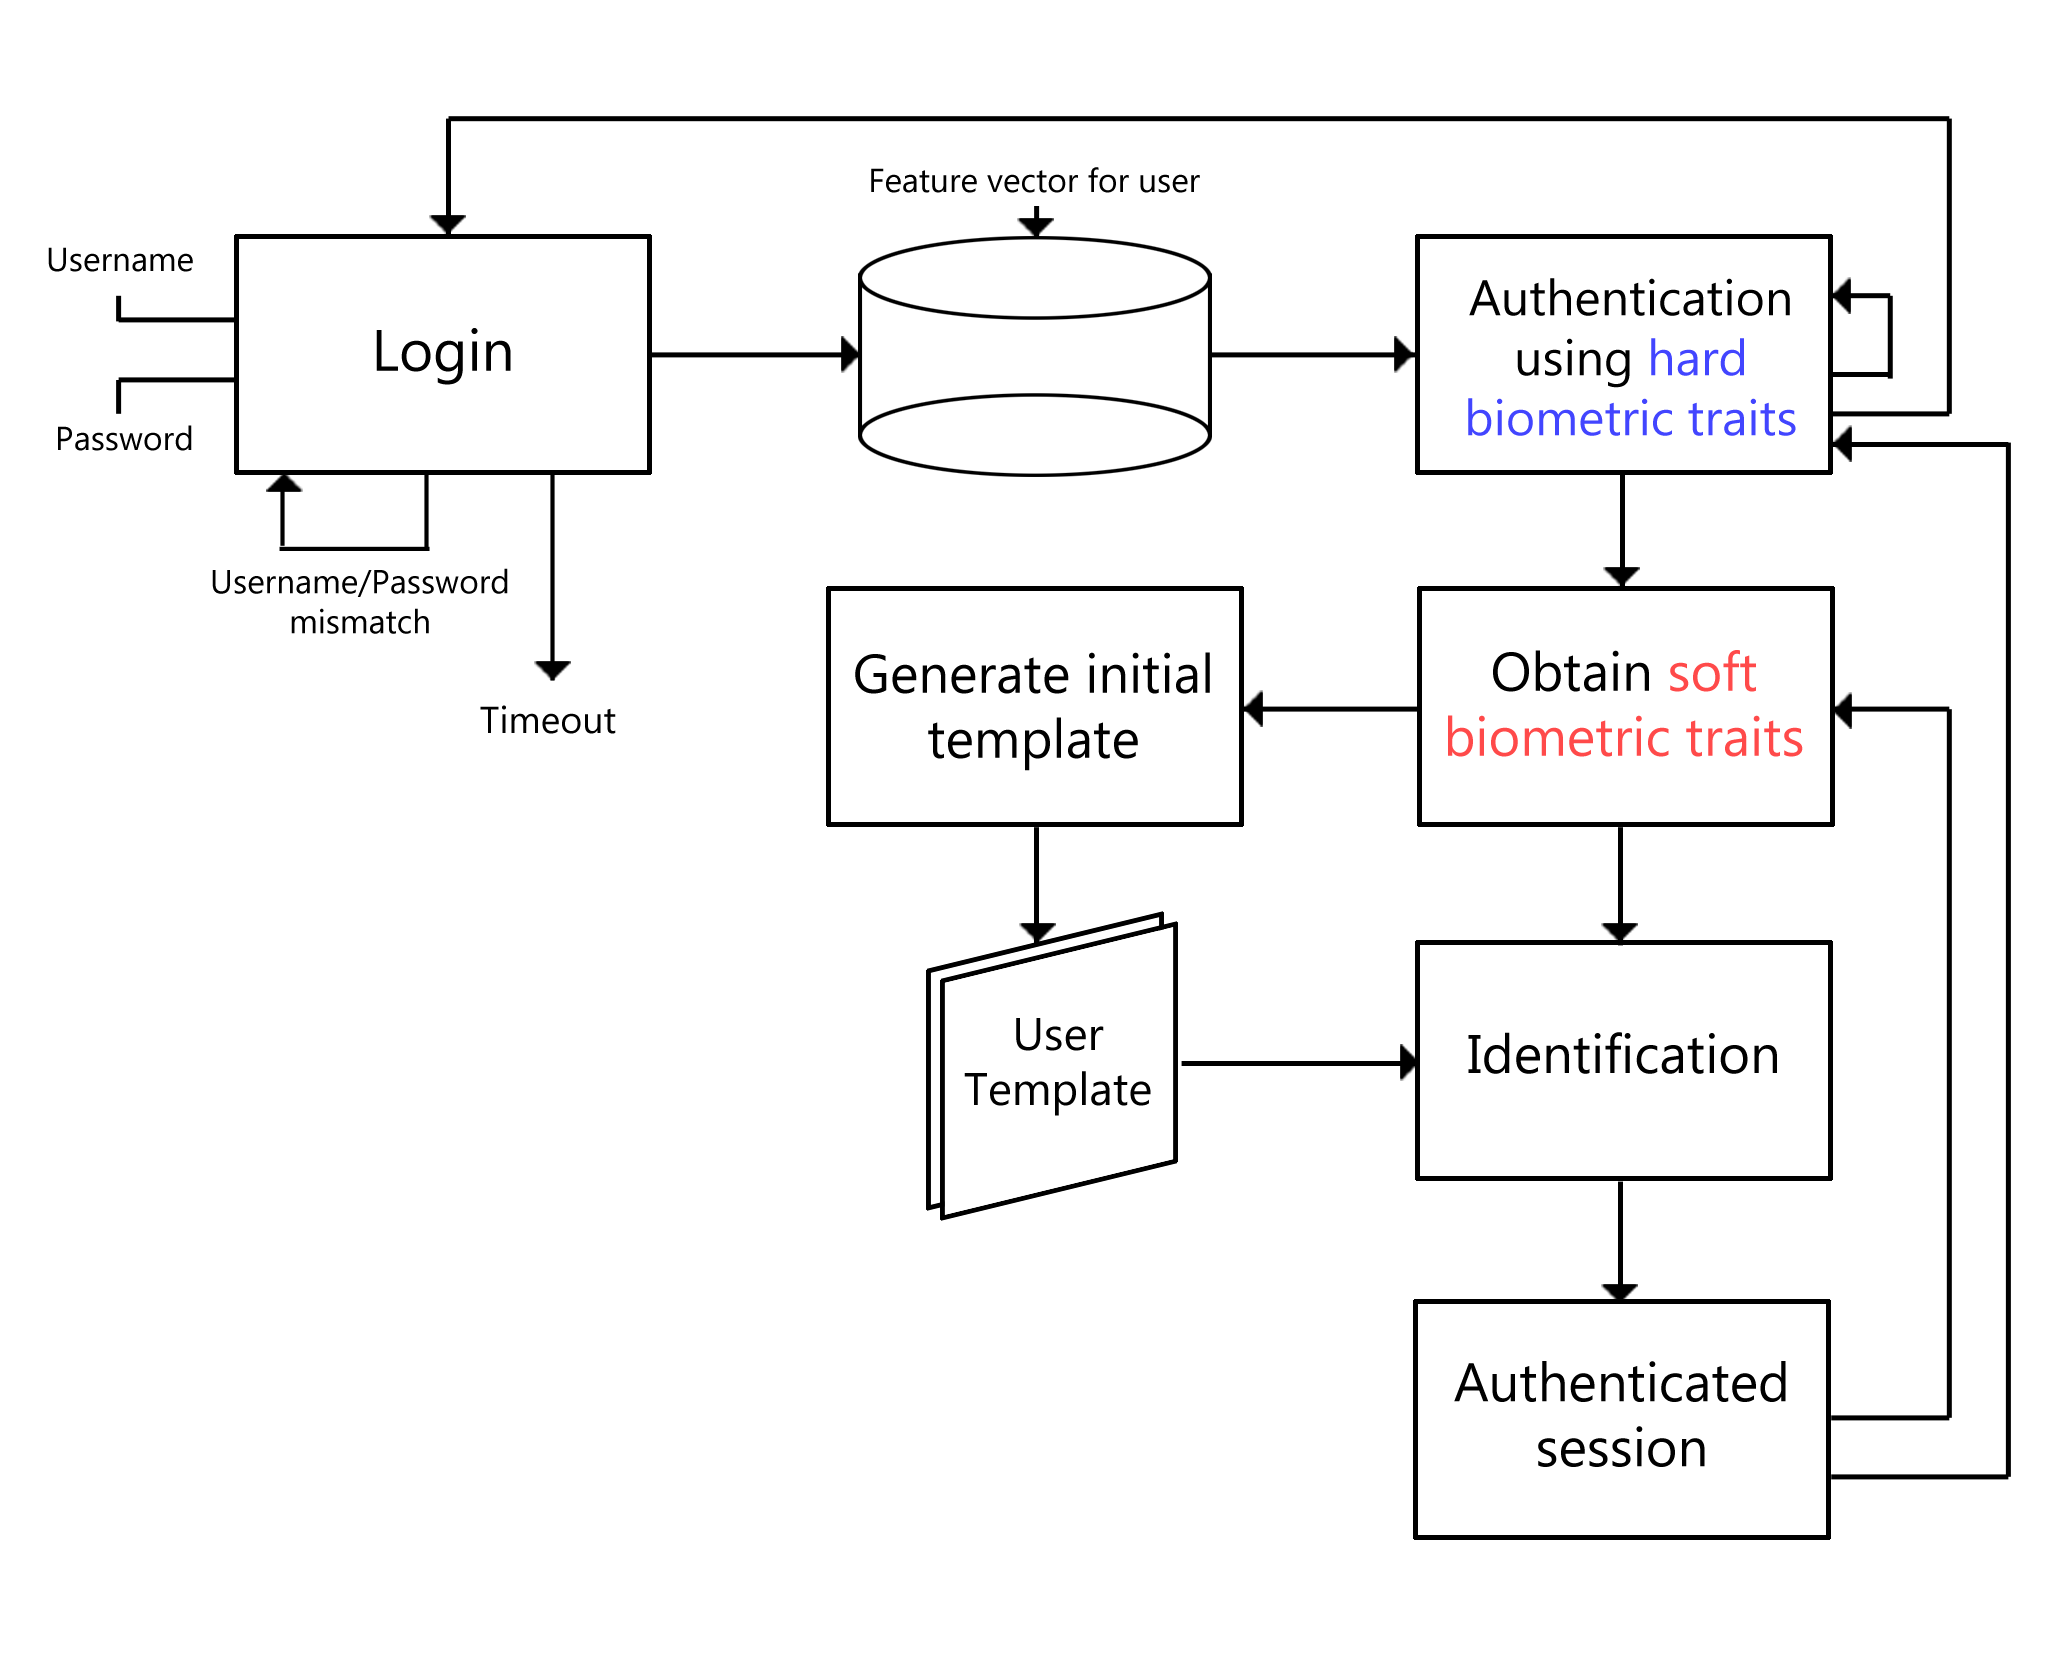
\includegraphics[scale=0.5]{img/overall_f.png}
	\caption{Continuous Authentication system overview}
	\label{fig:ca_overview}
\end{figure}
Each of these states is maintained by designing the respective modules as black-boxes, as seen in figure \ref{fig:ca_overview}.
The control flow moves between these states is based on the confidence of the authenticated user sitting in front of the system.
The modules which implementing these states are briefly described in the following sections.

\subsection{Conventional password}
The username-password pair is created during the account creation phase, during which the facial features of the user are also captured.
The password and the (automatically generated) user-id are encrypted and stored in the database.\\
At the time of login, the user is asked to enter the username-password pair, in order to satisfy the condition of \emph{something you know}.
The password entered is encrypted and compared to that stored in the database.
Hence, this phase can be viewed as a gatekeeper to the session. 

\subsection{Hard biometrics}
Once past the successful login phase, the control flow progresses into the hard biometrics mode.
In this phase, the traits unique to the user in front of the system is compared the parameters obtained during training, i.e, during the account creation phase.
The hard biometric traits captured by our proposed solution is restricted to facial features for two reasons:
\begin{itemize}
	\item To keep the cost of the system low.
	\item In case of more robust biometrics such as iris or fingerprint recognition, the user is required to deviate from the workflow. This hinders the system's ability to capture the required traits without disturbing the user. In contrast, by using facial features, the user can continue working in front of the system oblivious to the authentication process in the background.
\end{itemize}
However, the system is designed in such a way that any other hard biometric trait can be later added in form of a black-box. This requires the machine learning algorithm explained in the next section to be trained accordingly.
The hard biometrics phase hence satisfies the condition - \emph{something the user is}, hence providing a robust method of authenticating the user with high confidence during the session.\\
The facial recognition is achieved using the concept of Eigenfaces\cite{Turk91} as proposed by Turk and Pentland.
Although more complex solutions to face recognition such as Fisherface and neural networks are available, we show that Eigenfaces, even with drawbacks of comparatively lower accuracy and higher time required to process each frame can be overcome using the technique described in the next section.
Once again, the module implementing Eigenfaces can be easily subsituted for a more advanced algorithm, given that it predicts a user from a given image.
But, for the rest of the discussion, the module implementing face recognition implies Eigenface, in order to study a method to overcome the inherent noise from the hard biometrics module.

\subsection{Noise dampening}
If the output(confidence) produced by the hard biometrics mode is represented as the indicator function
$$ 1\{user_{recognized} = user_{authenticated}\} \in \{0,1\}$$,
the distribution of these outputs against time appears as shown in the the figure \ref{fig:no_svm}.
\begin{figure}[h!]
	\centering
	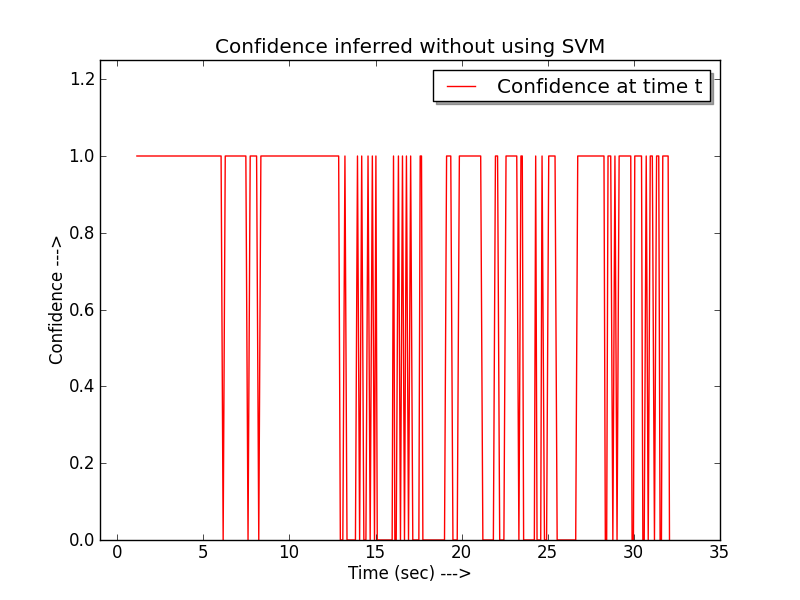
\includegraphics[scale=0.4]{img/no_svm.png}
	\caption{Output of Eigenfaces vs. time as described by the indicator function}
	\label{fig:no_svm}
\end{figure}
The information latent when the false negatives are produced is generally a result of:
\begin{itemize}
	\item A high degree of illumination changes in the surroundings
	\item Extreme movements and postures by the user, which maps to data not captured during training
\end{itemize}
Moreover, most face recognition algorithms, including Eigenfaces predicts the closest neighbour in the PCA subspace constructed using the training data.
This leads to a high probability of an imposter being authenticated when the training data is biased, such as in the case of very few registered users or the ratio of male-to-female is not balanced.\\
Our proposed technique overcomes these drawbacks, which applies to face recognition algorithms in general, by taking advantage of:
\begin{itemize}
	\item Temporal information and decaying old information
	\item Confidence in prediction of recognized face, which in case of Eigenfaces is the Mahalanobis distance of the projected point from its nearest neighbour
	\item Patterns inherent in the noise
\end{itemize}
The data extracted for these features from historical records is used to learn a classifier $y \in \{1,-1\}$, implemented as a Support Vector Machine. The outcome of this technique is continued in the results section.

\subsection{Soft biometrics}
Hard biometrics although being more robust and reliable than soft biometrics, falls short in three aspects\cite{Niin10}:
\begin{itemize}
	\item Required more time for processing each frame
	\item Restricts the user's postures and movements
	\item Falsely rejects user due to occlusion
\end{itemize}
These drawbacks are overcome at the expense of decrease in accuracy to satisfy the goal of not deviating the user from his usual work-flow. 
In our proposed solution, the soft biometric trait used is the shirt colour, but is extendable to other soft biometric forms of authentication such as complexion, gender\cite{Jain204}, etc. 


\section{Algorithms and techniques used}

\subsection{Face Detection using Viola-Jones algorithm}
The face detector proposed by Paul Viola and Micheal Jones\cite{Viola01} combines four key concepts\cite{servo}:
\begin{itemize}
	\item Simple rectangular features, called Haar features
	\item An Integral Image for rapid feature detection
	\item A variant of the learning algorithm AdaBoost
	\item Cascaded architecture
\end{itemize}
The features that Viola and Jones used are based on Haar wavelets.
Haar wavelets are single wavelength square waves (one high interval and one low interval).
In two dimensions, a square wave is a pair of adjacent rectangles - one light and one dark.
The actual rectangle combinations used for visual object detection are not true Haar wavlets.
Instead, they contain rectangle combinations better suited to visual recognition tasks.
Because of that difference, these features are called Haar features, or Haarlike features, rather than Haar wavelets.
The presence of a Haar feature is determined by subtracting the average dark-region pixel value from the average light-region pixel value.
If the difference is above a threshold (set during learning), that feature is said to be present.\\
To determine the presence or absence of hundreds of Haar features at every image location and at several scales efficiently, Viola and Jones used a technique called an Integral Image.
Using this technique, rectangular features can be evaluated in constant time, which gives them a considerable speed advantage over their more sophisticated relatives.\\
Viola and Jones combined a series of AdaBoost classifiers as a filter chain, that's especially efficient for classifying image regions.
Each filter is a separate AdaBoost classifier with a fairly small number of weak classifiers.
The cascade architecture has interesting implications for the performance of the individual classifiers. Because the activation of each classifier depends entirely on the behavior of its predecessor, the false positive rate for an entire cascade is:
\begin{equation}
F = \prod _{i=1}^{K} f_i
\end{equation}
Similarly, the detection rate is:
\begin{equation}
D = \prod _{i=1}^{K} d_i
\end{equation}
Thus, to match the false positive rates typically achieved by other detectors, each classifier can get away with having surprisingly poor performance. At the same time, however, each classifier needs to be exceptionally capable if it is to achieve adequate detection rates.

\subsection{Face Recognition using Eigenfaces}

\subsubsection{Face recognition using Eigenfaces}
Eigenfaces is a face recognition algorithm that was first described by Turk and Pentland in their paper published in 1991. It works to capture the variations present among the images of faces, that form the training set. It uses this information to create a face model where each image is represented as an eigenvector in what is called a "PCA subspace". Recognition of a test face is carried out by converting the test image into a similar eigenvector and then comparing its distance from all others in the subspace. The person corresponding to closest image is said to be the person recognized in the test image. It encodes the complete face characteristics, as opposed to capturing features of the face separately.\\

\subsubsection{ Eigenface generation }
Eigenfaces works in the following manner:
\begin{enumerate}
	\item A training set of images {\bf S} containing $\tau_{1},\tau_{2},..\tau_{M}$ total faces of the users to be recognized is prepared. These faces are captured during account creation of a user and converted to grayscale and equalized and resized to a standard resolution. Each image is converted to a vector of size {\bf N} by concatenating all the pixels row by row. These vectors are put into a matrix {\bf T} with each row representing an image.
	\item The average of all vectors $\psi$ is calculated and subtracted from each of the vectors in {\bf T} to obtain $\phi_{i}, i = 1,2,..,n$.
	\item The eigenvectors $u_{k}$ and eigenvalues $\lambda_{k}, k = 1,..,M$ of the co-variance matrix {\bf C} are calculated. The covariance matrix itself is found by: 
\begin{equation}
{\bf C} = \frac{1}{M}\sum_{n=1}^{M}\phi_{n}\phi_{n}^{T}
\end{equation}
	\item Since the dimension of C is very high (of the order of the number of pixels in the image), another matrix {\bf L} with the dimensions $MxM$ is constructed, 
\begin{equation}
{\bf L} = {\bf A}^{T}{\bf A}
\end{equation}
where 
\begin{equation}
{\bf A} = \{\phi_{1},\phi_{2},..,\phi_{M}\}
\end{equation}
	\item The eigenvectors v_{l} of the matrix {\bf L} are determined such that,
\begin{equation}
u_{l} = sum_{k=1}^{M}v_{lk}\phi_{k} 
\end{equation}
where $l = 1,..,M$.
\end{enumerate}

To recognize a face, the face image is transformed into its eigenface components. The input image $\tau_{new}$ is compared with the mean image and their difference is multiplied with each eigenvector of the {\bf L} matrix. Each value represents a weight and would be saved on a vector \Omega.
\begin{equation}
\omega_{k} = u_{k}^{T}(\tau_{new} - \psi)	\Omega^{T} = [\omega_{1},\omega_{2},..,\omega_{k}] 
\end{equation}

The Euclidiean distance $\varepsilon$ is minimized to determine which face class the new face belongs to. It is computed as follows:
\begin{equation}
\varepsilon_{k} = \parallel\Omega - \Omega_{k}\parallel 
\end{equation}

If $\varepsilon_{k}$ is below an established threshold $\theta_{\varepsilon}$, then the input face is considered to belong to that respective class.

\subsection{Noise Dampening using Support Vector Machines}
Using the output produced by the face recogntion module, the goal is to dampen the noise, by taking advantage of certain features like
\begin{itemize}
	\item Temporal information and decaying old information
	\item Confidence in prediction of recognized face, which in case of Eigenfaces is the Mahalanobis distance of the projected point from its nearest neighbour
	\item Patterns inherent in the noise
\end{itemize}
This is achieved by training a classifier on existing data:
\begin{equation}
\mathcal {D} = \{(x^{(1)},y^{(1)}),(x^{(2)},y^{(2)}),\ldots,(x^{(m)},y^{(m)})\}
\end{equation}
where $(x^{(i)}, y^{(i)})$ represents the $i^{th}$ training example in a set of $m$ training examples and $x \in \mathbb{R}^n, y \in \{+1, -1\}$. We generate a hyperplane represented as:
\begin{equation}
h_{w,b}(x) = g(w^Tx + b)
\end{equation}
where
\begin{equation}
g(z) = \left\{
\begin{array}{l l}
+1 & \quad \textit{if $z \geq 0$}\\
-1 & \quad \textit{if $z < 0$}\\
\end{array} \right.
\end{equation}
The (primal)optimization problem for finding the optimal margin classifier can be stated as:
\begin{equation}
\min_{\gamma, w, b} \frac{1}{2}\parallel w \parallel ^2\\
\end{equation}
subject to the constraint
\begin{equation}
y^{(i)}(w^Tx + b) \geq i = 1, ..., m
\end{equation}
When we construct the Langrangian for this optimization problem, we have:
\begin{equation} \label{eq:lang}
\mathcal {L}(w, b, \alpha) = \frac{1}{2} \parallel w \parallel ^2 - \sum_{i=1}^{m} \alpha_i [y^{(i)}(w^Tx^{(i)} + b) - 1]
\end{equation}
where $\alpha_{i}$ is a Langrange multiplier. To minimize $\mathcal{L}$, we differentiate this equation with respect to $w$ and $b$ to obtain:
\begin{equation} \label{eq:w}
w = \sum_{i=1}^{m} \alpha_{i} y^{(i)} x^{(i)}
\end{equation}
\begin{equation} \label{eq:ay}
\sum_{i=1}^{m} \alpha_{i} y^{(i)} = 0
\end{equation}
Plugging this back into equation \ref{eq:lang}, we get
\begin{equation}
\mathcal {L}(w, b, \alpha) = \sum_{i=1}^{m} \alpha_i - \frac{1}{2} \sum_{i,j=1}^{m} y^{(i)}y^{(j)}\alpha_i \alpha_j (x^{(i)})^T x^{(j)}
\end{equation}
Putting this together with the constraint $\alpha_i \geq 0$, we obtain the following the dual optimization problem:
\begin{equation} \label{eq:dual}
\max_{\alpha} W(\alpha) = \sum_{i=1}^{m} \alpha_i - \frac{1}{2} \sum_{i,j=1}^{m} y^{(i)}y^{(j)}\alpha_i \alpha_j \langle x^{(i)}, x^{(j)}\rangle
\end{equation}
subject to the constraints
% % % % % % % % % % % % % % % % % % % % % % % % % % % % 
% Implementation
% % % % % % % % % % % % % % % % % % % % % % % % % % % % 
\section{Implementation}


% % % % % % % % % % % % % % % % % % % % % % % % % % % % 
% Results
% % % % % % % % % % % % % % % % % % % % % % % % % % % % 
\section{Results}


% % % % % % % % % % % % % % % % % % % % % % % % % % % % 
% Conclusion and Future enhancements
% % % % % % % % % % % % % % % % % % % % % % % % % % % % 
\section{Conclusion and Future enhancements}

% do the biliography:
\bibliographystyle{IEEEbib}
\begin{thebibliography}{77}
\bibitem{Turk91} M. Turk and A. Pentland.
"Face recognition using eigenfaces."
\emph{Proc. IEEE Conference on Computer Vision and Pattern Recognition.} pp. 586-591.

\bibitem{Viola01}Paul Viola, Michael Jones.
"Robust Real-time Object Detection."
\emph{Second International Workshop on Statistical and Computational Theories of Vision - Modeling, Learning, Computing, and Sampling (Vancouver, Canada)}, July 13, 2001.

\bibitem{Niin10} Niinuma, K., Unsang Park, Fujitsu Labs. Ltd., Kawasaki, Japani, A.K. Jain
"Soft Biometric Traits for Continuous User Authentication" 
\emph{Information Forensics and Security, IEEE Transactions on}, 2010

\bibitem{Jain04}A.K. Jain, S.C. Dass, K. Nandakumar.
"Soft Biometric Traits for Personal Recognition Systems."
\emph{International Conference on Biometric Authentication}, 2004.

\bibitem{Klos00}Andrew J. Klosterman, Gregory R. Ganger.
"Secure Continuous Biometric-Enhanced Authentication", 
Carnegie Mellon University, Tech. Rep. CMU-CS-00-134, 2000.

\bibitem{Jain204}A. K. Jain, S. C. Dass, and K. Nandakumar,
“Can soft biometric traits assist user recognition?”,
Proc. SPIE, vol. 5404, pp. 561–572, 2004.

\bibitem{libsvm}Chang, Chih-Chung and Lin, Chih-Jen,
LIBSVM: A library for support vector machines,
\emph{ACM Transactions on Intelligent Systems and Technology}
available at \url{http://www.csie.ntu.edu.tw/~cjlin/libsvm}

\bibitem{servo}How face detection works,
\href{http://www.servomagazine.com/}{SERVO Magazine}, 2007

\bibitem{ann99}Anne Adams and Martina Angela Sasse.
Dec,1999/Vol.42.No.12, Communications ofthe ACM,
P40-Parker, D.B. Restating the foundation of information security-- In G.C.
Gable and W.J. Caelli, Eds., IT Security: The Need for International Cooperation.
Elsevier Science Publishers, Holland, 1992

\bibitem{war02} Ware, Karl.
Biometrics and strong authentication McGraw-Hill Osborne

\bibitem{john03}John Woodward, Nicholas M. Orlans, Peter T. Higgins.
Biometrics and strong authentication,McGraw-Hill Inc, 2003

\bibitem{bert96}A. Bertillon,
Signaletic Instructions including the theory and practice of Anthropometrical Identification, R.W.
McClaughry Translation, The Werner Company, 1896.

\bibitem{way97}J. L. Wayman,
“Large-scale Civilian Biometric Systems - Issues and Feasibility,” in Proceedings of Card Tech /
Secur Tech ID, 1997.

\bibitem{mon00}
F. Monrose and A. D. Rubin, 
“Keystroke dynamics as biometrics for authentication,” 
Future Generation Comput. Syst., vol. 16, pp.351–359, 2000.

\bibitem{turk03}
A. Altinok and M. Turk, 
“Temporal integration for continuous multi-modal biometrics,”
in Proc. Workshop on Multimodal User Authentication, 2003, pp. 131–137.

\bibitem{sim07}
T. Sim, S. Zhang, R. Janakiraman, and S. Kumar, 
“Continuous verification using multimodal biometrics,” 
IEEE Trans. Pattern Anal. Mach. Intell., vol. 29, no. 4, pp. 687–700, Apr. 2007.

\bibitem{azz08}
A. Azzini, S. Marrara, R. Sassi, and F. Scotti, “A fuzzy approach to
multimodal biometric continuous authentication,” Fuzzy Optimal De-
cision Making, vol. 7, pp. 243–256, 2008.
\bibitem{azz082}
A. Azzini and S. Marrara, “Impostor users discovery using a multi-
modal biometric continuous authentication fuzzy system,” Lecture
Notes in Artificial Intelligence, vol. 5178, pp. 371–378, 2008.
\bibitem{kang06}
H.-B. Kang and M.-H. Ju, “Multi-modal feature integration for secure
authentication,” in Proc. Int. Conf. Intelligent Computing, 2006, pp.
1191–1200.
\bibitem{car03}
C. Carrillo, “Continuous Biometric Authentication for Authorized Air-
craft Personnel: A Proposed Design,” Master’s thesis, Naval Postgrad-
uate School, Monterey, CA, 2003.

\end{thebibliography}


% where ``my-bibliography-file.bib'' is the name of the file with all the 
% BibTeX entries.

% do the biographies...
% \begin{biography}{Gregory L. Plett}
%   A bio with no face...
% \end{biography}

% If you want a picture with your biography, then specify the name of
% the postscript file in square brackets. That is, uncomment the
% following three lines and change the name of "face.ps" to the name of 
% your file.
%\begin{biography}[face.ps]{Gregory L. Plett}
%  A bio with a face...
%\end{biography}

%----------------------------------------------------------------------
% FIGURES
%----------------------------------------------------------------------
% There are many ways to include figures in the text. We will assume
% that the figure is some sort of EPS file.
%
% The outdated packages epsfig and psfig allow you to insert figures
% like: \psfig{filename.eps} These should really be done now using the
% \includegraphics{filename.eps} command.  
%
% i.e.,
%
% \includegraphics{file.eps}
%
% whenever you want to include the EPS file 'file.eps'. There are many
% options for the includegraphics command, and are outlined in the
% on-line documentation for the "graphics bundle". Using the options,
% you can specify the height, total height (height+depth), width, scale,
% angle, origin, bounding box "bb",view port, and can trim from around
% the sides of the figure. You can also force LaTeX to clip the EPS file
% to the bounding box in the file. I find that I often use the scale,
% trim and clip commands.
% 
% \includegraphics[scale=0.6,trim=0 0 0 0,clip=]{file.eps}
% 
% which magnifies the graphics by 0.6 (If I create a graphics for an
% overhead projector transparency, I find that a magnification of 0.6
% makes it look much better in a paper), trims 0 points off
% of the left, bottom, right and top, and clips the graphics. If the
% trim numbers are negative, space is added around the figure. This can
% be useful to help center the graphics, if the EPS file bounding box is
% not quite right.
% 
% To center the graphics,
% 
% \begin{center}
% \includegraphics...
% \end{center}
% 
% I have not yet written good documentation for this, but another 
% package which helps in figure management is the package ieeefig.sty,
% available at: http://www-isl.stanford.edu/people/glp/ieee.shtml
% Specify:
% 
%\usepackage{ieeefig} 
% 
% in the preamble, and whenever you want a figure,
% 
% \figdef{filename}
% 
% where, filename.tex is a LaTeX file which defines what the figure is.
% It may be as simple as
% 
% \inserteps{filename.eps}
%
% or
% \inserteps[includegraphics options]{filename.eps}
% 
% or may be a very complicated LaTeX file. 

\end{document}
